% ---------------------------------------------------------------------
% LaTeX template for abstract submission to EUROMECH Colloquium #609
%
% 7-aug-2019 m. uhlmann
% ---------------------------------------------------------------------
\documentclass[a4paper,11pt]{article}

%\usepackage[latin1]{inputenc}
%\usepackage[T1]{fontenc}
\usepackage[utf8]{inputenc}
\usepackage{subcaption}
\usepackage[paper=a4paper,left=28mm,right=28mm,top=25mm,bottom=30mm]{geometry}
\usepackage[pdftex,colorlinks=true,linkcolor=blue,citecolor=blue,urlcolor=blue]{hyperref}
\usepackage{graphicx}
\usepackage{epstopdf}
\usepackage[sort&compress,round]{natbib}
\usepackage{doi}
\usepackage{tikz}
 \usetikzlibrary{fit,arrows.meta,shapes.arrows}
\usepackage{fancyhdr}
\pagestyle{fancy}
\setlength{\headheight}{30pt}
\fancyhfoffset{32pt}
\lhead{}
\chead{%\bf
  \sffamily
  \parbox[t]{.96\linewidth}{
  \small
    ~ EUROMECH Colloquium 654 
    ``Bio-Inspired Fluid-Structure Interaction'' ~~~~~~~~~~~~
    9-11 July 2025, Vienna, Austria
  }
}
\rhead{}

\begin{document}

\vspace{-1.0cm}

\epstopdfsetup{suffix=}
%----------------------------------------------------------------------
\title{Wake Flow Control via Flexible Foils on a D-Shaped Body}

\author{Juan D'Adamo$^{1,2}$ \and Verónica Raspa $^3$ \and Ramiro Godoy-Diana$^{4}$\\
  $^1$  Universidad de Buenos Aires, Facultad de Ingenier\'ia, \\LFD, CONICET,Buenos Aires, Argentina\\
$^2$ Instituto Franco-Argentino de Dinámica de Fluidos para el Medio Ambiente,\\ IRL 2027, CNRS, UBA, CONICET, Buenos Aires, Argentina.\\
  $^3$ Universidad de Buenos Aires, Facultad de Ciencias Exactas y Naturales,\\  IFIBA, CONICET,   Buenos Aires,  Argentina.\\
  $^4$ Physique et Mécanique des Milieux Hétérogènes, \\ESPCI Paris-PSL (PMMH, UMR 7636), France  
}
\date{}
\maketitle

Drag forces in wake flows account for a significant portion of energy consumption in many industrial applications, particularly in transportation. Effective flow control strategies require a thorough understanding of the physical mechanisms that characterize wake flows. Active control methods involve introducing energy into the flow (e.g., through mobile parts, blowing, or suction), while passive control methods modify the flow by altering geometry, material, or surface properties.


Wake flows are typically characterized by the well-known Bénard-Von Kármán (BvK) instability, which generates a periodic vortex street pattern. We propose to modify this flow pattern through a special configuration of flexible foils attached to the surface of a bluff body producing significant drag reductions. 	On a recent work, \cite{garcia2021drag} obtained drag reductions that can be applied to a better aerodynamical design of trucks using a similar configuration. 	
 These reductions are attributed to foil reconfiguration \cite{gosselin2010drag} and changes in the hydrodynamic stability properties \citep{strykowski1990formation,Giannetti:2007p127,thiria2009passive}. However, flutter instability may also arise, increasing fluid inertial forces and potentially restraining drag reduction as discussed by \cite{leclercq2018does}.
		 
	
	In the present work, we experimentally study the strong fluid-structure interaction (FSI) for a D-shaped body with flexible foils in a wind tunnel as depicted by Figure \ref{fig_setup}. We characterize the modifications to the BvK vortex street caused by foil reconfiguration and wake-induced vibrations. Specifically, we examine whether small-amplitude fluttering can enhance drag reduction by altering the wake dynamics. With these results, we aim to contribute to the development of efficient aerodynamic designs, ultimately reducing energy consumption.
	
	

\begin{figure}
	
\begin{subfigure}[b]{.5\textwidth}
	\begin{tikzpicture}
	\node(fig) at (0,0){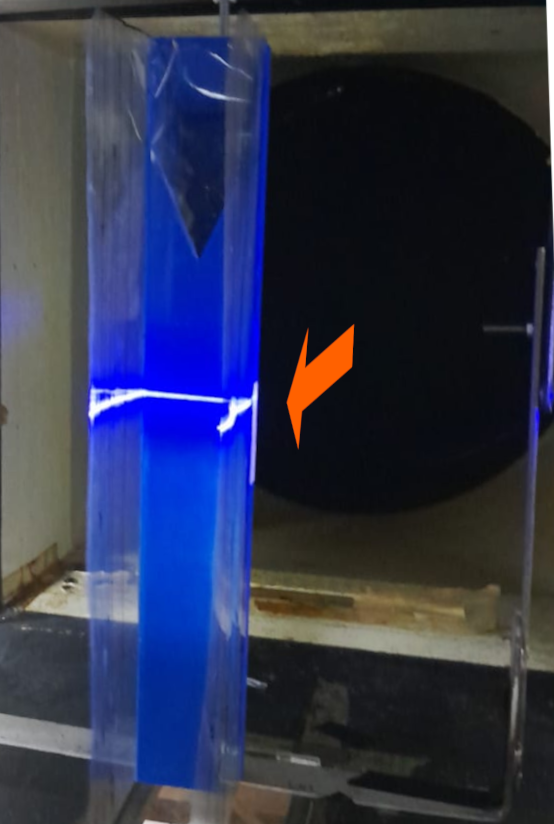
\includegraphics[width=0.9\textwidth,trim=0 1.5cm  0 2cm,clip]{./tunel_dshape_flex}};	
	
%\node[single arrow,   very thick, fill=orange,
%minimum width = 10pt, single arrow head extend=3pt,
%minimum height=20mm,
%rotate=230] at (fig) {};	
	
	\end{tikzpicture}
\subcaption{ }	
\end{subfigure}	
\begin{subfigure}[b]{.5\textwidth}
	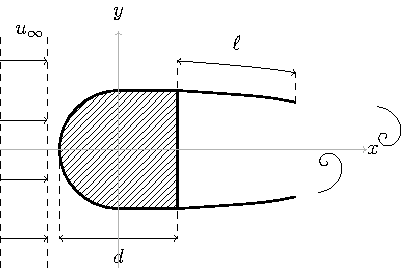
\includegraphics[width=\textwidth]{./setup_scheme}
	\subcaption{ }
\end{subfigure}
\label{fig}
\vspace{-0.5cm}
\caption{(a) Dshape with flexible foils in the wind tunnel. (b) Schematic diagram of the flow and solid configuration.}\label{fig_setup}
\end{figure}

% -----------------------------------------------------------------------
\bibliography{/home/juan/Documents/bibtex/citas.bib}
\bibliographystyle{plainnat}
\setlength{\bibsep}{.5ex}
%
% There are two ways to produce a list of references. 
%
% A) include a bibtex file:
%
% \bibliography{/home/uhlmann/TEX/bib/books.bib}
%
% B) insert the bibliography items directly:
%
 
%----------------------------------------------------------------------
\end{document}
% ---------------------------------------------------------------------